\documentclass[12pt]{report}

% Packages
%--------------------------------------------------

% General
%

\usepackage[T1]{fontenc}
\usepackage[utf8]{inputenc}
\usepackage[english]{babel}

% Layout
%

\usepackage[
    letterpaper,
    margin = 1in
]{geometry}
\usepackage{enumitem}
\usepackage{fancyhdr}
\usepackage{titlesec}

% Math
%

\usepackage{amssymb}
\usepackage{amsfonts}

% Graphics
%

\usepackage{newtxtext, newtxmath} % Times New Roman.
\usepackage{xcolor}
\usepackage{graphicx}
\usepackage{hyperref}

% Debugging
%

% \usepackage{showframe}

% Includes
%--------------------------------------------------

% Graphics
%--------------------------------------------------

\graphicspath{{./assets/img}}

% Colors
%--------------------------------------------------

\definecolor{Primary}{RGB}{172,43,55}
\definecolor{Accent}{RGB}{0,0,0}
\definecolor{Gray}{RGB}{169,176,183}
\definecolor{Body}{RGB}{52,56,59}

% \newcommand{\ColorBox}[3]{\tikz{\path[draw=#1,fill=#1] (0,0) rectangle (#2,#3);}}
\newcommand{\ColorBox}[3]{\textcolor{#1}{\rule{#2}{#3}}}

% Tables
%--------------------------------------------------

\UseTblrLibrary{varwidth}
\SetTblrInner[tblr]{measure=vbox}

% Fonts
%--------------------------------------------------

\newfontfamily{\MinionPro}[
    Path           = {./assets/fonts/minion_pro/},
    Extension      = .otf,
    UprightFont    = {MinionPro-Regular},
    ItalicFont     = {MinionPro-It},
    FontFace       = {md}{n}{MinionPro-Medium},
    FontFace       = {md}{it}{MinionPro-MediumIt},
    FontFace       = {sb}{n}{MinionPro-Semibold},
    FontFace       = {sb}{it}{MinionPro-SemiboldIt},
    BoldFont       = {MinionPro-Bold},
    BoldItalicFont = {MinionPro-BoldIt}
]{MinionPro}

\newfontfamily{\MyriadPro}[
    Path           = {./assets/fonts/myriad_pro/},
    Extension      = .otf,
    UprightFont    = {MYRIADPRO-REGULAR},
    ItalicFont     = {MYRIADPRO-IT},
    FontFace       = {sb}{n}{MYRIADPRO-SEMIBOLD},
    FontFace       = {sb}{it}{MYRIADPRO-SEMIBOLDIT},
    BoldFont       = {MYRIADPRO-BOLD},
    BoldItalicFont = {MYRIADPRO-BOLDIT}
]{MyriadPro}

\setmainfont{SourceSerifPro}[
    Path           = {./assets/fonts/source_serif_pro/},
    Extension      = .ttf,
    UprightFont    = {SourceSerifPro-Regular},
    ItalicFont     = {SourceSerifPro-Italic},
    % FontFace       = {md}{n}{SourceSerifPro-Medium},
    % FontFace       = {md}{it}{SourceSerifPro-MediumItalic},
    FontFace       = {sb}{n}{SourceSerifPro-SemiBold},
    FontFace       = {sb}{it}{SourceSerifPro-SemiBoldItalic},
    BoldFont       = {SourceSerifPro-Bold},
    BoldItalicFont = {SourceSerifPro-BoldItalic}
]

\newcommand{\FontVariant}[1]{\fontseries{#1}\selectfont}

\DeclareRobustCommand{\mddseries}{\FontVariant{md}}
\DeclareRobustCommand{\sbseries}{\FontVariant{sb}}
\DeclareTextFontCommand{\textmdd}{\mddseries}
\DeclareTextFontCommand{\textsb}{\sbseries}

% Miscellaneous
%--------------------------------------------------

\newcommand{\HRule}[1]{\rule{\linewidth}{#1}}
\pagestyle{fancy}

\fancyhf{}

\setlength{\headheight}{15pt}

\renewcommand{\chaptermark}[1]{\markboth{\textit{Chapter \arabic{chapter}.} #1}{}}
\renewcommand{\sectionmark}[1]{\markright{\textit{Section \arabic{section}.} #1}}

\fancyhead[L]{\leftmark}
\fancyhead[R]{\rightmark}
\fancyfoot[R]{\thepage}
\titleformat{\chapter}[hang]
    {\normalfont\huge\bfseries}
    {\thechapter}{20pt}{\huge}
\titlespacing*{\chapter}{0pt}{0pt}{40pt}

\titleformat{\section}[hang]
    {\normalfont\Large\bfseries}
    {\thesection}{20pt}{\Large}
\titlespacing*{\section}{0pt}{30pt}{20pt}

\titleformat{\subsection}[hang]
    {\normalfont\large\bfseries}
    {\thesubsection}{20pt}{\large}
\titlespacing*{\subsection}{0pt}{30pt}{20pt}

\titleformat{\subsubsection}[hang]
    {\normalfont\normalsize\bfseries}
    {\thesubsubsection}{20pt}{\normalsize}
\titlespacing*{\subsubsection}{0pt}{15pt}{10pt}

\newcommand{\Chapter}[2]{\chapter{#1}\label{ch:#2}}
\newcommand{\Section}[3]{\section{#1}\label{ch:#2:sec:#3}}
\newcommand{\SubSection}[4]{\subsection{#1}\label{ch:#2:sec:#3:subsec:#4}}
\newcommand{\SubSubSection}[5]{\subsubsection{#1}\label{ch:#2:sec:#3:subsec:#4:subsubsec:#5}}

\WithSuffix\newcommand\Chapter*[2]{\chapter*{#1}\label{ch:#2}\markboth{#1}{}\addcontentsline{toc}{chapter}{\nameref{ch:#2}}}

% Document
%--------------------------------------------------

\begin{document}

    \begin{titlepage}
        \centering
        
\includegraphics[]{wpi_logo.png} \\
        \vspace{1in}
        {\LARGE\textbf{Library Technology}} \\
        \vspace{1in}
        \begin{tabular}{c@{\hspace{5em}}c}
            {\large\scshape Participants} & {\large\scshape Advisors} \\
            \\
            Scanlon, Brandon              & Heineman, George \\
            Yasuna, Oliver
        \end{tabular} \\
        \vfill
        \today \\
        \vspace{0.5cm}
        \textit{This report represents work of one or more WPI undergraduate students submitted to the faculty as evidence of a degree requirement. WPI routinely publishes these reports on its web site without editorial or peer review.}
    \end{titlepage}

    \tableofcontents

    \chapter*{Abstract}
    \label{ch:abstract}
    \markboth{Abstract}{}
    \addcontentsline{toc}{chapter}{\nameref{ch:abstract}}

        ABSTRACT

    \chapter*{Executive Summary}
    \label{ch:executive_summary}
    \markboth{Executive Summary}{}
    \addcontentsline{toc}{chapter}{\nameref{ch:executive_summary}}

        EXECUTIVE SUMMARY

    \chapter*{Authorship}
    \label{ch:authorship}
    \markboth{Authorship}{}
    \addcontentsline{toc}{chapter}{\nameref{ch:authorship}}

        AUTHORSHIP

    \Chapter{Introduction}{introduction}
        %Introduction
The George C. Gordon Library is a vital part of the college experience at Worcester Polytechnic Institute. The library staff work tirelessly to maintain and reinforce quality educational services, as well as strive to help students directly with boundless academic concerns. The staff utilize various web-based product suites to host and organize the various services they offer. However, many library staff members view some of these products as counterproductive and challenging to operate efficiently within.

Simply put, the library staff use these tools daily and have found numerous issues that are of high demand to be solved. For example, LibraryH3lp, a popular tool among libraries, is often reported to have bugs and that it is rather difficult to use. Additionally, the library staff utilizes a handful of the products from SpringShare. Nonetheless, these tools often prove to perform unreliably and cause more problems than they solve.

Despite the challenges posed by these tools, the library staff continue to work hard to provide the best possible service to WPI students. They are constantly trying to find new and improved ways to work around the challenges presented by these tools. Therefore, we sought to step in with this project to ease the troubles that the WPI library staff encounter.

Both participants of this MQP together completed a closely related IQP. The IQP's goal was to develop a mobile application for the Gordon Library that collects the library's most commonly used services into one convenient place. With the extensive research and feedback the Gordon Library's staff provided us during our IQP, we began our MQP with ample information about the systems that worked and those that did not.

The LibraryH3lp platform was reportedly riddled with pitfalls pertaining to the user's experience on both the administrative and client sides which needed more functionality for what the Gordon Library required to best provide students with quality educational services. A change was in order to match the standard of what the library continually aims to maintain with the tools they used. This project set out to implement a solution to such problems, thus developing a web application that would replace LibraryH3lp and its current library chat application. We used the existing application as a foundation for reference of features and capabilities to then build an overhauled version that included a number of improvements tailored to what the library staff had detailed.

We organized a number of meetings with the library staff during this project. Our initial meeting during the beginning of the project was used to establish a solid baseline to best structure the issues with the current system. From there, could build a skeleton of the system we were planning to develop along with storyboards in an adolescent state. Then, we held a second meeting with the library staff once these storyboards were completely fleshed out. During this meeting we discussed and reinforced the concepts that were brainstormed at the beginning of the project and demonstrate them though storyboards. The feedback on them was positive and we received additional options we may have, though just out of the scope of our jurisdiction, but would enhance our application even more.

    \Chapter{Literature Review}{literature_review}
        LITERATURE REVIEW

    \Chapter{Methodology}{methodology}
        INTRODUCTION

\Section{Needs Analysis}{methodology}{needs_analysis}
    NEEDS ANALYSIS

\Section{Feasibility Study}{methodology}{feasibility_study}
    FEASIBILITY STUDY

\Section{Technology}{methodology}{technology}
    TODO

\SubSection{Frontend}{methodology}{technology}{frontend}
    TODO: Talk about web application.

\SubSubSection{Languages}{methodology}{technology}{frontend}{languages}

    For frontend development, we chose to use web technologies.
    This means that our application bundle will use web languages such as JavaScript, HTML, and CSS.
    To provide a better development experience and to catch more bugs in compile time, we will use TypeScript over JavaScript whenever possible.
    TypeScript, unlike JavaScript, is strongly and statically typed.
    Statically typed languages are used throughout the Computer Science program at WPI.
    It is best that we apply these programming teachings in our MQP.
    We will also use Sass over CSS whenever possible.
    Sass is a CSS preprocessor that compiles into plain CSS.
    Sass makes it possible to write reusable functions and mixins for styles.

\SubSubSection{Frameworks}{methodology}{technology}{frontend}{frameworks}

    We chose to use Angular to build our web application.
    Specifically, Angular version 14, the latest major version as of this writing.
    Angular is a component-based framework for building web applications.
    The Angular family offers almost everything that we needed to build a scalable chat platform.
    We designed and implemented custom components with the look-and-feel according to \hyperref[ch:methodology:sec:conceptual_designs:subsec:wpi_guidelines]{WPI guidelines}.

\SubSection{Middle-tier}{methodology}{technology}{middletier}
    TODO: Explain what middle-tier is. Pretend the audience are monkeys.

\SubSubSection{Languages}{methodology}{technology}{middletier}{languages}

    We chose to use Java as our primary languages for writing the middle-tier.
    Java is the primary language used in WPI Computer Science courses.
    Both MQP participants have professional experience using the language.

\SubSubSection{Frameworks}{methodology}{technology}{middletier}{frameworks}

    Spring and Spring Boot was used to build our middle-tier.
    Spring is a mature framework for building applications.
    It offers all of the tools necessary to implement a complete middle-tier.

\SubSubSection{Tools}{methodology}{technology}{tools}{frameworks}

    We used the OpenAPI 3 (Swagger) standard to design the API for the library chat platform.

\SubSection{Server}{methodology}{technology}{server}
    We worked closely with WPI's Information Technology department to create a Linux server for the MQP.
The server runs on Ubuntu Server 22.04.

\SubSubSection{Web Server}{methodology}{technology}{server}{web_server}

    We used Apache HTTP Server to serve our web application.
    This decision was made to stay consistent with the web server used by other groups at WPI.

\SubSubSection{Database}{methodology}{technology}{server}{database}

    PostgreSQL was our choice of database.
    While WPI's Computer Science courses utilize Oracle or SQL Server, we chose PostgreSQL because of our familiarity with it and its capabilities.


\SubSection{DevOps}{methodology}{technology}{devops}
    TODO: Explain DevOps to non-nerds.

\SubSubSection{Continuous Integration}{methodology}{technology}{devops}{ci}

    Continuous Integration (CI) is the practice of automating the process of integrating code changes into software.
    Since there were only two developers part of the MQP and we are not running a multi-billion-dollar company, we did not need to establish a complex CI.
    We chose to simply use GitHub Actions.
    Development commits (to non-\texttt{main} branches) compiled and deployed to a staging URL.
    Production commits (to the \texttt{main} branch) compiled and deployed to the main URL.


\Section{Use Cases}{methodology}{use_cases}
    % This section offers a list of use cases.
% These use cases outline the flow of events for functionality on the platform.
% Our use case format is based on one provided by \href{https://www.usability.gov/how-to-and-tools/methods/use-cases.html}{usability.gov}.

% \SubSection{From Contact Us Page}{methodology}{use_cases}{contact_us}
%     This section offers use cases that usually start with the Client on the "Contact Us" page.


%--------------------------------------------------------------------------------------
\UseCaseNew{Visit Library Hours Page}{visit_library_hours_page}{%
    Describes the process when a User acquires the library's operating hours.
}{%
    \FakeItem User
}{%
    \FakeItem The User is on the Contact Us page.
}{%
    \FakeItem The User requests the library's operating hours.
}{%
    \FakeNumberedItem{1} The User navigates to the library's operating hours link. \par
    \FakeNumberedItem{2} The User is redirected to the library's operating hours.
}{%
    The library hours are displayed to the User.
}
%-------------------------------------------------------------------------------------
\UseCaseNew{Visit News \& Events Page}{visit_news_and_events_page}{%
    Describes the process when a User acquires the library's current news and upcoming events.
}{%
    \FakeItem User
}{%
    \FakeItem The User is on the Contact Us page.
}{%
    \FakeItem The User requests information about news \& events.
}{%
    \FakeNumberedItem{1} The User navigates to the library's news \& events link.\par
    \FakeNumberedItem{2} The User is redirected to the library's news \& events page.
}{%
    The news \& events are displayed to the User.
}
%--------------------------------------------------------------------------------------
\UseCaseNew{Visit Tech Suite Booking page}{visit_tech_suite_booking_page}{%
    Describes the process when a User views Tech Suite Booking information.
}{%
    \FakeItem User
}{%
    \FakeItem The User is on the Contact Us page.
}{%
    \FakeItem The User requests information about Tech Suite Booking.
}{%
    \FakeNumberedItem{1} The User navigates to the Tech Suite Booking link. \par
    \FakeNumberedItem{2} The User is redirected to the Tech Suite Booking page.
}{%
    Tech Suite Booking information is displayed to the User.
}
%-------------------------------------------------------------------------------------
\UseCaseNew{Visit Alumni Information Page}{visit_alumni_information_page}{%
    Describes the process when a User views information regarding Alumnae.
}{%
    \FakeItem User
}{%
    \FakeItem The User is on the Contact Us page.
}{%
    \FakeItem The User requests information about Alumni.
}{%
    \FakeNumberedItem{1} The User navigates to the Alumni Information link. \par
    \FakeNumberedItem{2} The User is redirected to the Alumni Information page.
}{%
    Alumni information is displayed to the User.
}
%-------------------------------------------------------------------------------------
\UseCaseNew{Visit FAQs Page}{visit_faqs_page}{%
     Describes the process when a User views the answers to questions commonly asked.
}{%
    \FakeItem User
}{%
    \FakeItem The User is on the Contact Us page.
}{%
    \FakeItem The User requests answers to frequently asked questions.
}{%
    \FakeNumberedItem{1} The User navigates to the Frequently Asked Questions link. \par
    \FakeNumberedItem{2} The User is redirected to the Frequently Asked Questions page.
}{%
    Frequently asked questions and their answers are displayed to the User.
}
%------------------------------------------------------------------------------------
\UseCaseNew{Visit Research A Topic Page}{visit_research_a_topic_page}{%
    Describes the process when a User acquires assistance with researching a topic.
}{%
    \FakeItem User
}{%
    \FakeItem The User is on the Contact Us page.
}{%
    \FakeItem The User requests information about researching a topic.
}{%
    \FakeNumberedItem{1} The User navigates to the Research A Topic link. \par
    \FakeNumberedItem{2} The User is redirected to the Research A Topic Page.
}{%
    Researching a topic information is displayed to the User.
}
%------------------------------------------------------------------------------------
\UseCaseNew{Visit Library Chat}{visit_library_chat}{%
    Describes the process when a User acquires assistance from a librarian.
}{%
    \FakeItem User
}{%
    \FakeItem The User is on the Contact Us page.
}{%
    \FakeItem The User requests to chat with a librarian. 
}{%
    \FakeNumberedItem{1} The User navigates to the Chat With A Librarian link. \par
    \FakeNumberedItem{2} The User is redirected to the Question Specification page. \par
    \FakeNumberedItem{3} The User navigates to the Create Chatroom link. \par
    \FakeNumberedItem{4} The User is paired with a librarian.
}{%
    A librarian joins the User's chatroom to help and answer the User's question.
}
%------------------------------------------------------------------------------------



% \SubSection{Chatroom Creation}{methodology}{use_case}{chatroom_creation}
%     This section offers use cases that start with the Client on the "Question Specification" page.


%--------------------------------------------------------------------------------------
\UseCaseNew{Choose Remain Anonymous}{choose_remain_anonymous}{%
     Describes the process when a User chooses whether or not to remain anonymous while chatting with a librarian.
}{%
    \FakeItem User
}{%
    \FakeItem The User is authenticated and authorized. \par
    \FakeItem The User is on the Question Specification page.
}{%
    \FakeItem The User is requesting to remain anonymous in the proceeding chatroom.
}{%
    \FakeNumberedItem{1} The User navigates to the Remain Anonymous checkbox. \par
    \FakeNumberedItem{2} The User checks the Remain Anonymous checkbox. \par
    \FakeNumberedItem{3} The User's chatting preference is set to anonymous.
}{%
    The User's name is displayed as anonymous while chatting.
}
%-------------------------------------------------------------------------------------
\UseCaseNew{Choose Question Category/Subcategory}{choose_question_category_and_subcategory}{%
     Describes the process when a User chooses the appropriate category that best fits their question.
}{%
    \FakeItem User
}{%
    \FakeItem The User is authenticated and authorized. \par
    \FakeItem The User is on the Question Specification page.
}{%
    \FakeItem The User is requesting a specific question category for the chatroom.
}{%
    \FakeNumberedItem{1} The User navigates to the Question Categories dropdown menu. \par
    \FakeNumberedItem{2} The User selects the appropriate category. \par
    \FakeNumberedItem{3} The User responds to the appropriate category specifiers.
}{%
    The User's question category is appropriately set for chat sorting.
}
%-------------------------------------------------------------------------------------
\UseCaseNew{Write Brief Description}{write_brief_description}{%
     Describes the process when a User writes a brief description of their question.
}{%
    \FakeItem User
}{%
    \FakeItem The User is authenticated and authorized. \par
    \FakeItem The User is on the Question Specification page.
}{%
    \FakeItem The User provides a brief description.
}{%
    \FakeNumberedItem{1} The User navigates to the Brief Description entry field. \par
    \FakeNumberedItem{2} The User inputs a response.
}{%
    \FakeItem The User's brief description is displayed as the first chat in the chatroom. \par
    \FakeItem The User's brief description is displayed in the chat pool for the admins.
}
%-------------------------------------------------------------------------------------
\UseCaseNew{Create Chatroom}{create_chatroom}{%
        Describes the process when a user create a new chatroom.
    }{%
        \FakeItem User
    }{%
        \FakeItem The User has the authority to create a chatroom. \par
        \FakeItem The User has provided the proper information for \hyperref[uc:choose_remain_anonymous]{remaining anonymous}, \hyperref[uc:choose_question_category_and_subcategory]{selecting an appropriate question category and subcategory}, as well as providing a \hyperref[uc:write_brief_description]{brief description}.
    }{%
        \FakeItem The User requests to create a chatroom.
    }{%
        \FakeNumberedItem{1} The User creates the chatroom. \par
        \FakeNumberedItem{2} The librarians are invited to the chatroom. \par
        \FakeNumberedItem{3} Use case \hyperref[uc:join_chatroom]{Join Chatroom}.
    }{%
        The chatroom is displayed for the User.
    }
%-------------------------------------------------------------------------------------

% \SubSection{Chatroom Actions}{methodology}{use_cases}{chatroom_actions}
%     Use cases that describe functionality of chatrooms.

\SubSubSection{General}{methodology}{use_cases}{chat_platform}{general}

    \UseCaseNew{User Archive Chatroom}{user_archive_chatroom}{%
        Describes the process when a user archives a chatroom.
    }{%
        \FakeItem Initiating User \par
        \FakeItem Other Participating Users
    }{%
        \FakeItem The Initiating User has the authority to archive a chatroom.
    }{%
        \FakeItem The Initiating User requests to archive a chatroom.
    }{%
        \FakeNumberedItem{1} The Initiating User archives the chatroom. \par
        \FakeNumberedItem{2} The display is updated for all actors. \par
        \FakeNumberedItem{3} A sound is played for all actors. \par
        \FakeNumberedItem{4} A notification is sent to all actors.
    }{%
        The chatroom is archived and no actors can send messages.
    }

    \UseCaseNew{Automatically Archive Chatroom}{automatically_archive_chatroom}{%
        Describes the process when a chatroom is automatically archived due to a period of inactivity.
    }{}{%
        \FakeItem There is a period of inactivity in the chatroom.
    }{%
        \FakeItem A period of inactivity in the chatroom.
    }{%
        \FakeNumberedItem{1} The chatroom is archived. \par
        \FakeNumberedItem{2} The display is updated for all participating users. \par
        \FakeNumberedItem{3} A sound is played for all participating users. \par
        \FakeNumberedItem{4} A notification is sent to all participating users.
    }{%
        The chatroom is archived and no users can send messages.
    }

    \UseCaseNew{Restore Chatroom}{restore_chatroom}{%
        Describes the process when a user restores an archived chatroom.
    }{%
        \FakeItem Initiating User \par
        \FakeItem Other Participating Users
    }{%
        \FakeItem The Initiating User has the authority to restore a chatroom.
    }{%
        \FakeItem The Initiating User requests to restore an archived chatroom.
    }{%
        \FakeNumberedItem{1} The Initiating User restores the archived chatroom. \par
        \FakeNumberedItem{2} Use case \hyperref[uc:join_chatroom]{Join Chatroom}. \par
        \FakeNumberedItem{3} A notification is sent to all actors.
    }{%
        The chatroom is restored, users can send messages, and all users are aware of this.
    }

\SubSubSection{Participants}{methodology}{use_cases}{chat_platform}{participants}

    \UseCaseNew{Join Chatroom}{join_chatroom}{%
        Describes the process when a user joins a chatroom.
    }{%
        \FakeItem Initiating User \par
        \FakeItem Other Participating Users
    }{%
        \FakeItem The Initiating User has the authority to join a chatroom.
    }{%
        \FakeItem The Initiating User requests to join a chatroom.
    }{%
        \FakeNumberedItem{1} The Initiating User joins the chatroom. \par
        \FakeNumberedItem{2} The join action is timestamped. \par
        \FakeNumberedItem{3} The displays is updated for Other Participating Users. \par
        \FakeNumberedItem{4} A sound is played for all actors.
    }{%
        The Initiating User has joined the chatroom and all actors are aware of this.
    }

    \UseCaseNew{Leave Chatroom}{leave_chatroom}{%
        Describes the process when a user leaves a chatroom.
    }{%
        \FakeItem Initiating User \par
        \FakeItem Other Participating Users
    }{}{%
        \FakeItem The Initiating User requests to leave a chatroom.
    }{%
        \FakeNumberedItem{1} The Initiating User leaves the chatroom. \par
        \FakeNumberedItem{2} The leave action is timestamped. \par
        \FakeNumberedItem{3} The display is updated for all actors. \par
        \FakeNumberedItem{4} A sound is played for all actors.
    }{%
        The Initiating User has left the chatroom and all actors are aware of this.
    }

    \UseCaseNew{Invite User}{invite_user}{%
        Describes the process when a user invites another user to a chatroom.
    }{%
        \FakeItem Initiating User \par
        \FakeItem Invited User \par
        \FakeItem Other Participating Users
    }{%
        \FakeItem The Initiating User has the authority to invite another user to a chatroom.
    }{%
        \FakeItem The Initiating User requests to invite the Invited User to a chatroom.
    }{%
        \FakeNumberedItem{1} The Initiating User invites the Invited User to the chatroom. \par
        \FakeNumberedItem{2} The invite action is timestamped. \par
        \FakeNumberedItem{3} The Invited User is notified. They can now perform use case \hyperref[uc:join_chatroom]{Join Chatroom}. \par
        \FakeNumberedItem{4} The display is updated for the Initiating User and Other Participating Users.
    }{%
        The Invited User is invited to the chatroom and all actors are aware of this.
    }

    \UseCaseNew{Remove User}{remove_user}{%
        Describes the process when a user removes a user from a chatroom.
    }{%
        \FakeItem Initiating User \par
        \FakeItem Removed User - Can be the Initiating User. \par
        \FakeItem Other Participating Users
    }{%
        \FakeItem The Initiating User has the authority to remove a user from a chatroom.
    }{%
        \FakeItem The Initiating User requests to remove the Removed User from a chatroom.
    }{%
        \FakeNumberedItem{1} The Initiating User removes the Removed User from the chatroom. \par
        \FakeNumberedItem{2} The remove action is timestamped. \par
        \FakeNumberedItem{3} The display is updated for all actors.
    }{%
        The Removed User is removed from the chatroom and all actors are aware of this.
    }

\SubSubSection{Messages}{methodology}{use_cases}{chat_platform}{messages}
    
    \UseCaseNew{Send Message}{send_message}{%
        Describes the process when a user sends a message.
    }{%
        \FakeItem Initiating User \par
        \FakeItem Other Participating Users
    }{%
        \FakeItem The Initiating User is in a chatroom. \par
        \FakeItem The Initiating User has the authority to send a message. \par
        \FakeItem The Initiating User's message is not blank.
    }{%
        \FakeItem The Initiating User requests to send a message.
    }{%
        \FakeNumberedItem{1} The Initiating User sends the message. \par
        \FakeNumberedItem{2} The message is timestamped. \par
        \FakeNumberedItem{3} The Initiating User's message box is cleared. \par
        \FakeNumberedItem{4} The message is appended to the end of the transcript for all actors.
    }{%
        The Initiating User's message is appended to the end of the transcript.
    }
    
    \UseCaseNew{Receive Message}{receive_message}{%
        Describes the process when a user receives a message.
    }{%
        \FakeItem User
    }{%
        \FakeItem The User is in a chatroom.
    }{}{%
        \FakeNumberedItem{1} The chatroom transcript is updated on the display. \par
        \FakeNumberedItem{2} A sound is played.
    }{%
        The chatroom transcript has been updated.
    }

    \UseCaseNew{Read Message}{read_message}{%
        Describes the process when a user reads a message.
    }{%
        \FakeItem Initiating User \par
        \FakeItem Other Participating Users
    }{%
        \FakeItem The Initiating User is in a chatroom.
    }{%
        \FakeItem The Initiating User reads a message.
    }{%
        \FakeNumberedItem{1} The Initiating User reads the message. \par
        \FakeNumberedItem{2} The read action is timestamped. \par
        \FakeNumberedItem{3} The transcript is updated for all actors to reflect that the Initiating User has read the message.
    }{%
        The chatroom transcript has been updated.
    }




% \SubSubSection{Client}{methodology}{use_cases}{chat_platform}{client}

%     \UseCase{Send Message}{send_message}{%
%         Describes the process when a Client sends a message to the Middle-Tier.
%     }{%
%         \FakeItem Client \par
%         \FakeItem Middle-Tier
%     }{%
%         \FakeNumberedItem{1} Client sends message to Middle-Tier. \par
%         \FakeNumberedItem{2} Client receives response from Middle-Tier. \par
%         \FakeNumberedItem{3} Client updates display.
%     }{%
%         Message is sent to Middle-Tier.
%     }{%
%         \FakeItem Client requests to send a message.
%     }{%
%         \FakeItem Client is in a chatroom. \par
%         \FakeItem Client's message body is not empty.
%     }
%     %-------------------------------------------------------------------------------------   
%     \UseCase{Fetch Messages}{fetch_messages}{%
%         Describes a process when a Client requests messages from the Middle-Tier.
%     }{%
%         \FakeItem Client \par
%         \FakeItem Middle-Tier
%     }{%
%         \FakeNumberedItem{1} Client requests messages from Middle-Tier. \par
%         \FakeNumberedItem{2} Client receives response from Middle-Tier. \par
%         \FakeNumberedItem{3} Client updates display.
%     }{%
%         All messages are displayed on the Client.
%     }{%
%         \FakeItem Client is in a chatroom. \par
%         \FakeItem 10 seconds have elapsed since previous request.

%     }{}
%     %-------------------------------------------------------------------------------------   
%     \UseCase{Fetch Read Receipts}{fetch_read_receipts}{%
%         Describes a process when a Client requests  from the Middle-Tier.
%     }{%
%         \FakeItem Client \par
%         \FakeItem Middle-Tier
%     }{%
%         \FakeNumberedItem{1} Client requests messages from Middle-Tier. \par
%         \FakeNumberedItem{2} Client receives response from Middle-Tier. \par
%         \FakeNumberedItem{3} Client updates display.
%     }{%
%         All messages are displayed on the Client.
%     }{%
%         \FakeItem Client is in a chatroom. \par
%         \FakeItem 10 seconds have elapsed since previous request.
%     }{}
%     %-------------------------------------------------------------------------------------   
%     \UseCase{New Chatroom}{new_chatroom}{%
%         Describes the process when a Client requests to create a new chatroom.
%     }{%
%         \FakeItem Client \par
%         \FakeItem Middle-Tier
%     }{%
%         \FakeNumberedItem{1} Client sends request to create a new chatroom to Middle-Tier. \par
%         \FakeNumberedItem{2} Client receives response from Middle-Tier.
%     }{%
%         \FakeItem Client is aware of the new chatroom.
%     }{%
%         \FakeItem Client requests to create a new chatroom.
%     }{}
%     %-------------------------------------------------------------------------------------   
%     \UseCase{Join Chatroom}{join_chatroom}{%
%         Describes the process when a Client requests to join an existing chatroom.
%     }{%
%         \FakeItem Client \par
%         \FakeItem Middle-Tier
%     }{%
%         \FakeNumberedItem{1} Client sends request to join an existing chatroom to Middle-Tier. \par
%         \FakeNumberedItem{2} Client receives response from Middle-Tier. \par
%         \FakeNumberedItem{3} Client updates display.
%     }{%
%         The chatroom is displayed on the Client.
%     }{%
%         \FakeItem Client requests to join an existing chatroom.
%     }{}
%     %-------------------------------------------------------------------------------------   
%     \UseCase{Invite Participant}{invite_participant}{%
%         Describes the process when a Client invites a participant.
%     }{%
%         \FakeItem Client \par
%         \FakeItem Middle-Tier
%     }{%
%         \FakeNumberedItem{1} Client sends request to add a participant to Middle-Tier. \par
%         \FakeNumberedItem{2} Client receives response from Middle-Tier. \par
%         \FakeNumberedItem{3} Client updates display.
%     }{%
%         All participants are displayed on the Client.
%     }{%
%         \FakeItem Client requests to add a participant.
%     }{%
%         \FakeItem Client is in a chatroom. \par
%         \FakeItem Client is librarian.
%     }
%     %-------------------------------------------------------------------------------------   
%     \UseCase{Leave Chatroom}{leave_chatroom}{%
%         Describes the process when a Client requests to leave a chatroom.
%     }{%
%         \FakeItem Client \par
%         \FakeItem Middle-Tier
%     }{%
%         \FakeNumberedItem{1} Client requests confirmation. \par
%         \FakeNumberedItem{2} Client sends request to leave a chatroom to Middle-Tier. \par
%         \FakeNumberedItem{3} Client receives response from Middle-Tier. \par
%         \FakeNumberedItem{4} Client updates display.
%     }{%
%         The chatroom is removed from the display on the Client.
%     }{%
%         \FakeItem Client requests to leave a chatroom.
%     }{%
%         \FakeItem Client is in a chatroom.
%     }

% \SubSubSection{Middle-Tier}{methodology}{use_cases}{chat_platform}{middle-tier}

%     \UseCase{Receive Message}{receive_message}{%
%         Describes the process when the Middle-Tier receives a message request.
%     }{%
%         \FakeItem Middle-Tier
%     }{%
%         \FakeNumberedItem{1} Middle-Tier sanitizes the message.
%                              If the message is a file, Middle-Tier performs security checks. \par
%         \FakeNumberedItem{2} Middle-Tier checks for vulgar content in the message. \par
%         \FakeNumberedItem{3} If the message passed all filters, Middle-Tier stores the message. \par
%         \FakeNumberedItem{4} Middle-Tier sends a response.
%     }{%
%         The message is stored.
%     }{%
%         \FakeItem Middle-Tier receives a message request.
%     }{%
%         \FakeItem Request is authentic and requester has the proper authority.
%     }
%     %-------------------------------------------------------------------------------------   
%     \UseCase{Provide Messages}{provide_messages}{%
%         Describes the process when the Middle-Tier receives a request for messages.
%     }{%
%         \FakeItem Middle-Tier
%     }{%
%         \FakeNumberedItem{1} Middle-Tier queries messages. \par
%         \FakeNumberedItem{2} Middle-Tier sends a response.
%     }{%
%         The messages are provided.
%     }{%
%         \FakeItem Middle-Tier receives a request for messages.
%     }{%
%         \FakeItem Request is authentic and requester has the proper authority.
%     }
%     %-------------------------------------------------------------------------------------  
%     \UseCase{Provide Read Receipts}{provide_read_receipts}{%
%         Describes the process when the Middle-Tier gets a request to provide read receipts.
%     }{%
%         \FakeItem Middle-Tier
%     }{%
%         \FakeNumberedItem{1} Middle-Tier queries read receipts. \par
%         \FakeNumberedItem{2} Middle-Tier sends a response.
%     }{%
%         The read receipts are provided.
%     }{%
%         \FakeItem Middle-Tier receives a request to provide read receipts.
%     }{%
%         \FakeItem Request is authentic and requester has the proper authority. \par
%         \FakeItem An unread message was received by the user.
%     }
%     %-------------------------------------------------------------------------------------
%     \UseCase{Provide Typing Statuses}{provide_typing_statuses}{%
%         Describes the process when the Middle-Tier gets a request to provide typing statuses.
%     }{%
%         \FakeItem Middle-Tier
%     }{%
%         \FakeNumberedItem{1} Middle-Tier receives a request to update typing statuses. \par
%         \FakeNumberedItem{2} Middle-Tier sends a response.
%     }{%
%         The typing statuses are updated.
%     }{%
%         \FakeItem Middle-Tier receives a request to provide typing statuses.
%     }{%
%         \FakeItem Request is authentic and requester has the proper authority. \par
%         \FakeItem User is typing in the chatroom.
%     }
%     %------------------------------------------------------------------------------------- 
%     \UseCase{Create Chatroom}{create_chatroom}{%
%         Describes the process when the Middle-Tier receives a request to create a new chatroom.
%     }{%
%         \FakeItem Middle-Tier
%     }{%
%         \FakeNumberedItem{1} Middle-Tier creates the chatroom. \par
%         \FakeNumberedItem{2} Middle-Tier sends a response.
%     }{%
%         The new chatroom is created.
%     }{%
%         \FakeItem Middle-Tier receives a request to create a new chatroom.
%     }{%
%         \FakeItem Request is authentic and requester has the proper authority.
%     }
%     %-------------------------------------------------------------------------------------
%     \UseCase{Add User To Chatroom}{add_user_to_chatroom}{%
%         Describes the process when the Middle-tier receives a request to add a user to a chatroom.
%     }{%
%         \FakeItem Middle-Tier
%     }{%
%         \FakeNumberedItem{1} Middle-Tier adds the user to the chatroom. \par
%         \FakeNumberedItem{2} Middle-Tier sends a response.
%     }{%
%         The user is added to the chatroom.
%     }{%
%         \FakeItem Middle-Tier receives a request to add a user to a chatroom.
%     }{%
%         \FakeItem Request is authentic and requester has the proper authority.
%         \FakeItem User is not already in the chatroom.
%     }
%     %-------------------------------------------------------------------------------------
%     \UseCase{Invite User To Chatroom}{invite_user_to_chatroom}{%
%         Describes the process when the Middle-tier receives a request to notify and invite a user to join a chatroom.
%     }{%
%         \FakeItem Middle-Tier
%     }{%
%         \FakeNumberedItem{1} Middle-Tier sends a notification to the invitee. \par
%         \FakeNumberedItem{2} Middle-Tier sends a response.
%     }{%
%         The user is notified and invited to join the chatroom.
%     }{%
%         \FakeItem Middle-Tier receives the request to notify and invite the user to the chatroom.
%     }{%
%         \FakeItem Request is authentic and requester has the proper authority.
%         \FakeItem User is not already in the chatroom.
%     }
%     %-------------------------------------------------------------------------------------
%     \UseCase{Remove User From Chatroom}{remove_user_from_chatroom}{%
%         Describes the process when the Middle-tier receives a request to remove a user from a chatroom.
%     }{%
%         \FakeItem Middle-Tier
%     }{%
%         \FakeNumberedItem{1} Middle-Tier removes the user from the chatroom. \par
%         \FakeNumberedItem{2} Middle-Tier sends a response.
%     }{%
%         The user is no longer in the chatroom.
%     }{%
%         \FakeItem Middle-Tier receives a request to remove a user from a chatroom.
%     }{%
%         \FakeItem Request is authentic and requester has the proper authority. \par
%         \FakeItem User is already in the chatroom.
%     }
%     %-------------------------------------------------------------------------------------  















% Status (Available, Away, Offline)
% Admin Kicking and signing out of others
% Blocking users from chatting options
% IP Tracking
% Data analytics
% Link to Outlook / Calendar
% Transcripts of chat after conclusion
% Speech to text
% Chat to email (Creating a case)
% Estimated wait time (User)
% Elapsed wait time (Admin)
% AFK timeout after 15 minutes
% AFK warning notification after X minutes
% Rejoinable chat is one party leaves. If everyone leaves a chat, the chat will close.
% Admin specified content filter (specific string. i.e. "F U C K")

% \UseCase{}{}{%
%     
% }{%
%     \FakeItem 
%     \FakeItem 
% }{%
%     \FakeNumberedItem{1}  \par
%     \FakeNumberedItem{2}  \par
%     \FakeNumberedItem{3}  \par
%     \FakeNumberedItem{4}  \par
%     \FakeNumberedItem{5}  \par
%     \FakeNumberedItem{6} 
% }{%
    
% }{%
%     \FakeItem 
% }{%
%     \FakeItem 
% }

% \SubSection{Chatroom Pool}{methodology}{use_cases}{chatroom_pool}
%     Use cases that describe functionality of the chatroom pool seen on the administrative side.

%--------------------------------------------------------------------------------------
\UseCaseNew{Receive Chatroom}{receive_chatroom}{%
     Describes the process when a User receives a chatroom.
}{%
    \FakeItem User
}{%
    \FakeItem The User has the property authority.
}{%
    \FakeItem \textit{Implicit}
}{%
    \FakeNumberedItem{1} The chatroom pool page is updated on the display. \par
    \FakeNumberedItem{2} A notification is sent to the User at 0, 60, 90, 120, etc. seconds.
}{%
    The chatroom pool page has been updated.
}
%--------------------------------------------------------------------------------------
\UseCaseNew{Set User Activity Status}{set_user_status}{%
     Describes the process when a User sets their activity status
}{%
    \FakeItem User
}{%
    \FakeItem The User has the proper authority.
}{%
    \FakeItem The User requests to change their activity status.
}{%
    \FakeNumberedItem{1} The User requests to change their activity status. \par
    \FakeNumberedItem{2} The User's activity status is changed and the display is updated.
}{%
    The User's activity status is updated accordingly.
}
%-------------------------------------------------------------------------------------
\UseCaseNew{Set Away Status}{set_away_status}{%
     Describes the process when a User has their status set to Away.
}{%
    \FakeItem User
}{%
    \FakeItem The User has the proper authority. \par
    \FakeItem The User has had no activity in the application for 10 minutes.
}{%
    \FakeItem The User has exceeded 10 minutes of inactivity.
}{%
    \FakeNumberedItem{1} The User has been inactive for 10 minutes. \par
    \FakeNumberedItem{2} The User's activity status is set to Away and the display is updated.
}{%
    The User's activity status is set to Away.
}
%-------------------------------------------------------------------------------------

\Section{Conceptual Designs}{methodology}{conceptual_designs}
    This sections discusses and demonstrates conceptual designs.

\SubSection{WPI Guidelines}{methodology}{conceptual_designs}{wpi_guidelines}
    WPI's Marketing \& Communications office offers clear guidelines for designs that represent the institution standards.
The guidelines highlight the power of consistency for all WPI representations and graphics.
Our final product aims to comply with the guidelines to the furthest extent possible.
From the Marketing \& Communications office:
% TODO: Cite.
\begin{displayquote}
    Marketing Communications offers a number of tools, templates, and self-serve resources to help the campus community create unified, branded, and targeted communications for your audiences.
\end{displayquote}
Read more about the guidelines and find more resources \href{https://www.wpi.edu/offices/marketing-communications/resources}{here}.

\SubSubSection{Color}{methodology}{conceptual_designs}{wpi_guidelines}{color}

    % TODO: Cite.
    % TODO: PMS glossary.
    % TODO: Pantone registered symbol.
    WPI's official colors use the Pantone Matching System (PMS).
    The colors are Crimson (PMS \texttt{187c}) and Gray (PMS \texttt{429c}).
    Black is used as an accent color.
    \textit{Note that colors in this document may be inaccurate due to colorspaces.}

    % TODO: Cite.
    \begin{Figure}{Table}{H}
        \centering
        \begin{tblr}{
            hlines,
            vlines
        }
            \textbf{Color}               & \textbf{Identifier}     & \textbf{Pantone} & \textbf{CMYK}        & \textbf{RGB}         & \textbf{HTML} \\
            \ColorBox{Primary}{1cm}{1cm} & Primary                 & \texttt{187c}    & \texttt{7,100,82,26} & \texttt{172,43,55}   & \texttt{ac2b37} \\
            \ColorBox{Accent}{1cm}{1cm}  & Accent                  &                  & \texttt{0,0,0,100}   & \texttt{0,0,0}       & \texttt{000000} \\
            \ColorBox{Gray}{1cm}{1cm}    & Gray                    & \texttt{429c}    & \texttt{21,11,9,23}  & \texttt{169,176,183} & \texttt{a9b0b7} \\
            \ColorBox{Body}{1cm}{1cm}    & Body                    &                  & \texttt{12,5,0,7}    & \texttt{52,56,59}    & \texttt{34383b} \\
        \end{tblr}
        \caption{WPI Colors}
        \label{fig:wpi_colors}
    \end{Figure}

\SubSubSection{Logos}{methodology}{conceptual_designs}{wpi_guidelines}{logos}

    % TODO.
    WPI LOGOS.

\SubSubSection{Fonts}{methodology}{conceptual_designs}{wpi_guidelines}{fonts}

    WPI guidelines specify two fonts: \href{https://fonts.adobe.com/fonts/minion}{Minion Pro} and \href{https://fonts.adobe.com/fonts/myriad}{Myriad Pro}.
    Minion Pro is used for formal, authoritative, and traditional text.
    Myriad Pro is used for informal, youthful, and friendly text.

    \begin{Figure}{Table}{H}
        \centering
        \begin{tblr}{
            hlines,
            vlines
        }
            \textbf{Font Family}     & Minion Pro                                      & Myriad Pro \\
            \textbf{Regular}         & {\MinionPro Minion Pro}                         & {\MyriadPro Myriad Pro} \\
            \textbf{Italic}          & {\MinionPro\itshape Minion Pro}                 & {\MyriadPro\itshape Myriad Pro} \\
            \textbf{Medium}          & {\MinionPro\FontVariant{md}Minion Pro} \\
            \textbf{Medium Italic}   & {\MinionPro\FontVariant{md}\itshape Minion Pro} \\
            \textbf{Semibold}        & {\MinionPro\FontVariant{sb}Minion Pro}          & {\MyriadPro\FontVariant{sb}Myriad Pro} \\
            \textbf{Semibold Italic} & {\MinionPro\FontVariant{sb}\itshape Minion Pro} & {\MyriadPro\FontVariant{sb}\itshape Myriad Pro} \\
            \textbf{Bold}            & {\MinionPro\FontVariant{bx}Minion Pro}          & {\MyriadPro\FontVariant{bx}Myriad Pro} \\
            \textbf{Bold Italic}     & {\MinionPro\FontVariant{bx}\itshape Minion Pro} & {\MyriadPro\FontVariant{bx}\itshape Myriad Pro} \\
        \end{tblr}
        \caption{WPI Font Families}
        \label{fig:wpi_font_families}
    \end{Figure}

    These fonts are utilized for different parts of brand content.

    % TODO: Cite.
    \begin{Figure}{Table}{H}
        \centering
        \begin{tblr}{
            hlines,
            vlines
        }
            % TODO: Fonts.
            \textbf{Identifier} & \textbf{Font}       & \textbf{Example} \\
            Formal Primary      & Minion Pro Semibold & {\MinionPro\FontVariant{sb}\color{Primary}ABCDEFGHIJKLMNOPQRSTUVWXYZ\\abcdefghijklmnopqrstuvwxyz\\1234567890} \\
            Formal Secondary    & Minion Pro Italic   & {\MinionPro\itshape\color{Primary}ABCDEFGHIJKLMNOPQRSTUVWXYZ\\abcdefghijklmnopqrstuvwxyz\\1234567890} \\
            Informal Secondary  & Myriad Pro Semibold & {\MyriadPro\FontVariant{sb}\color{Primary}ABCDEFGHIJKLMNOPQRSTUVWXYZ\\abcdefghijklmnopqrstuvwxyz\\1234567890} \\
            \SetCell[c=3]{c}\textbf{\itshape Specific Elements} \\
            Headline            & Minion Pro Semibold & {\MinionPro\FontVariant{sb}\color{Primary}Headline} \\
            Informal Headline   & Myriad Pro Semibold & {\MyriadPro\FontVariant{sb}\color{Primary}Informal Headline} \\
            Sub-headline        & Minion Pro Italic   & {\MinionPro\itshape\color{Primary}Sub-headline} \\
            Body                & Myriad Pro Regular  & {\MyriadPro\color{Body}Body}
        \end{tblr}
        \caption{WPI Font Usages}
        \label{fig:wpi_font_usages}
    \end{Figure}

\SubSection{Storyboards}{methodology}{conceptual_designs}{storyboards}
    
We put together a number of storyboards to best draw initial designs of the application. They were also used in a meeting with the library staff to exhibit our perspective on what the application will look and feel like. The below figure shows what would replace the current Contact Us page with which streamlines the user flow and routes users automatically with general questions rather than prompting a chatroom with a librarian for such questions.

\begin{figure}[H]
    \centering
    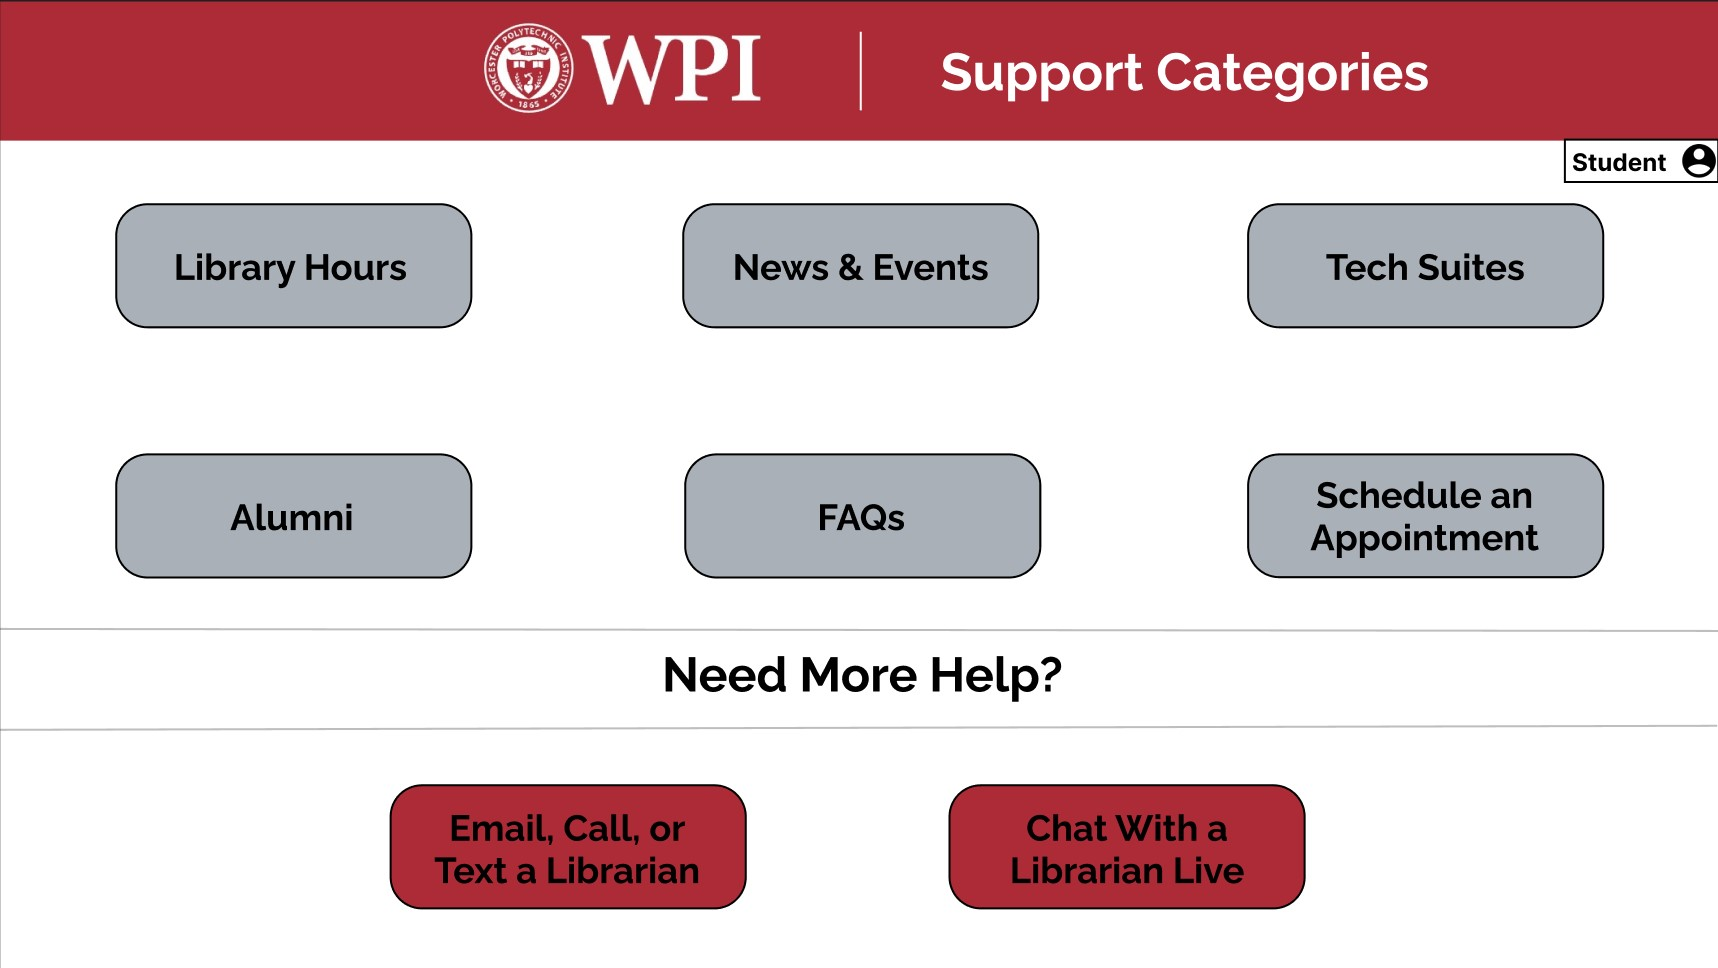
\includegraphics[width=0.5\textwidth]{chapters/methodology/conceptual_designs/MQP Main Page}
    \caption{Student view of the Contact Us page.}
\end{figure}

The figure below showcases a rudimentary iteration of what the chatroom interface is expected to look like. Here, from the librarian's perspective, the user is supplied with a number of convenient features ranging from automated prompt responses, chat duration, file uploading, and more.

\begin{figure}[H]
    \centering
    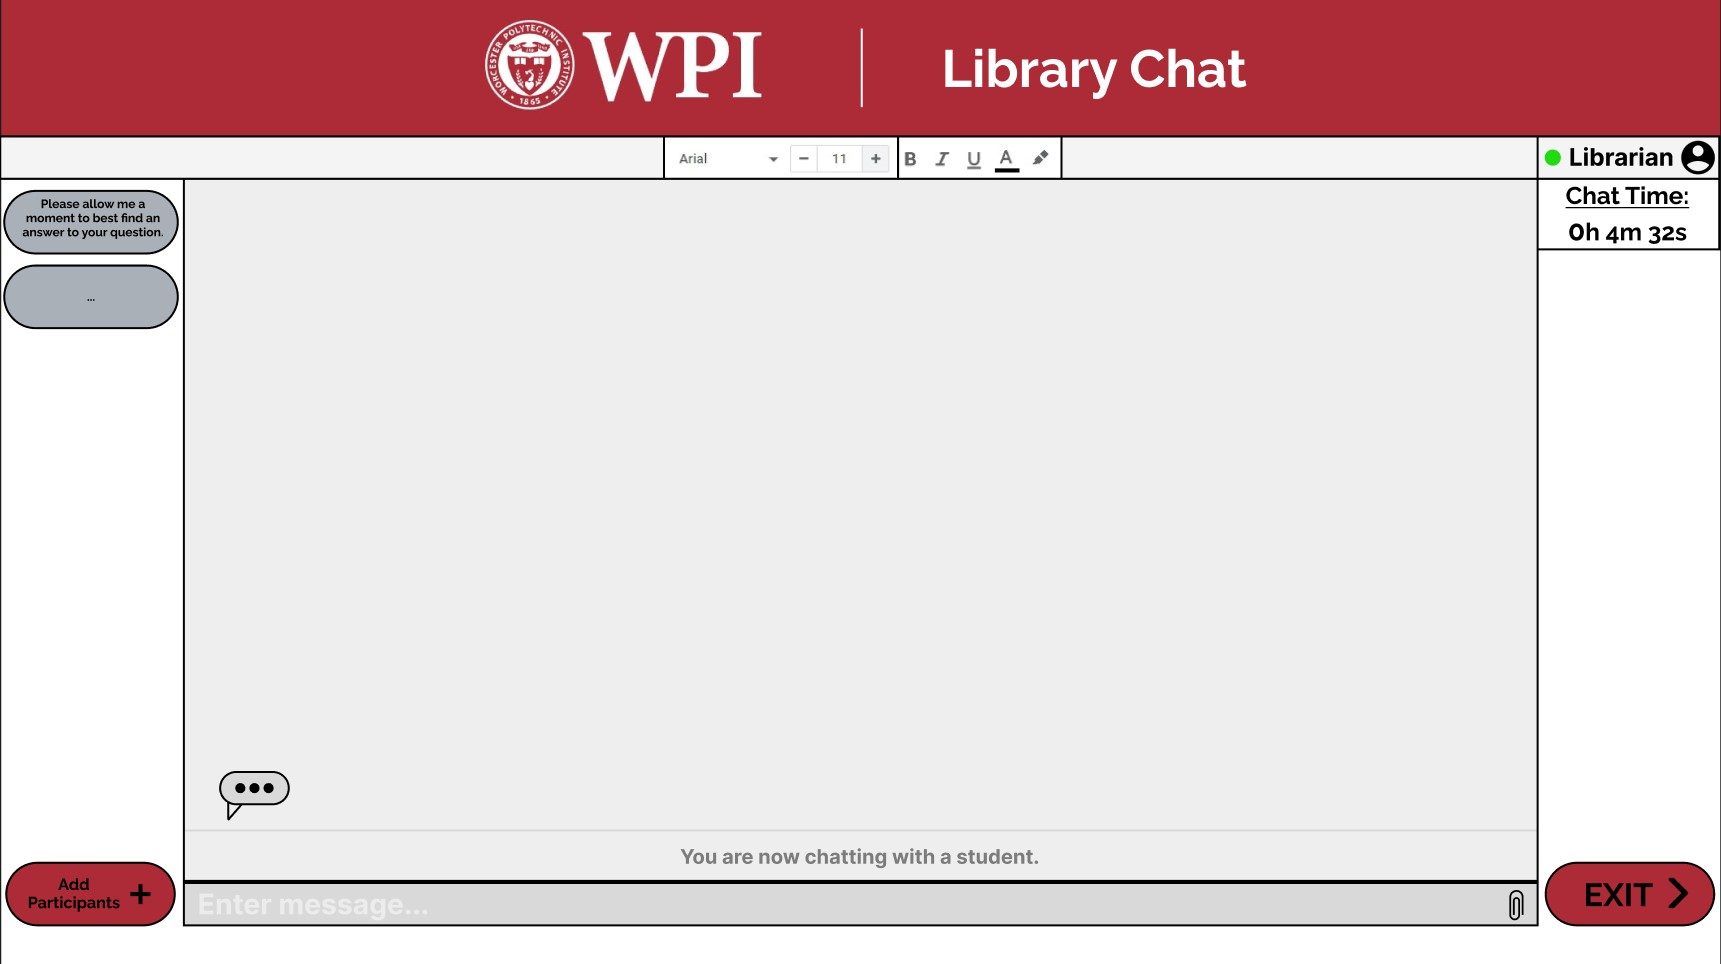
\includegraphics[width=0.5\textwidth]{chapters/methodology/conceptual_designs/MQP Librarian Chat.jpg}
    \caption{Librarian view of a chatroom.}
\end{figure}


\Section{Implementation Specifications}{methodology}{implementation_specifications}
    IMPLEMENTATION SPECIFICATIONS

\SubSection{New Chatroom Fields}{methodology}{implementation_specifications}{new_chatroom_fields}
    TODO

\begin{CompactItemize}
    \item \textbf{Category}\quad\textit{Select}
    \begin{CompactItemize}
        \item \textbf{Research}
        \begin{CompactItemize}
            \item \textbf{Type}\quad\textit{Select}
            \begin{CompactItemize}
                \item All sources
                \item Scholarly sources
                \item Non-scholarly sources
            \end{CompactItemize}
            \item \textbf{Subjects}\quad\textit{Multiselect}
            \begin{CompactItemize}
                % https://www.wpi.edu/academics/calendar-courses/course-descriptions
                \item Aerospace Engineering
                \item Air Force Aerospace Studies
                \item Architectural Engineering
                \item Bioinformatics \& Computational Biology
                \item Biology \& Biotechnology
                \item Biomedical Engineering
                \item Chemical Engineering
                \item Chemistry \& Biochemistry
                \item Civil, Environmental, \& Architectural Engineering
                \item Computer Science
                \item Data Science
                \item Electrical \& Computer Engineering
                \item Fire Protection Engineering
                \item Humanities \& Arts
                \item Interactive Media \& Game Development
                \item Manufacturing Engineering
                \item Materials Science \& Engineering
                \item Mathematical Sciences
                \item Mechanical \& Materials Engineering
                \item Military Science
                \item Physical Education
                \item Physics
                \item Robotics Engineering
                \item Social Science \& Policy Studies
                \item Systems Engineering
                \item Business
            \end{CompactItemize}
        \end{CompactItemize}
        \item \textbf{Books}
        \begin{CompactItemize}
            \item \textbf{Major Genre}\quad\textit{Select}
            \begin{CompactItemize}
                \item \textbf{All}
                \begin{CompactItemize}
                    \item \textbf{Genres}\quad\textit{Multiselect}
                    \begin{CompactItemize}
                        \item \hyperref[cco:fiction_genres]{\textbf{Fiction Genres}} + \hyperref[cco:nonfiction_genres]{\textbf{Non-fiction Genres}}
                    \end{CompactItemize}
                \end{CompactItemize}
                % https://blog.reedsy.com/book-genres/
                \item \textbf{Fiction}
                \begin{CompactItemize}
                    \item\label{cco:fiction_genres} \textbf{Genres}\quad\textit{Multiselect}
                    \begin{CompactItemize}
                        \item Fantasy
                        \item Science Fiction
                        \item Dystopian
                        \item Action \& Adventure
                        \item Mystery
                        \item Horror
                        \item Thriller \& Suspense
                        \item Historical Fiction
                        \item Romance
                        \item Women's Fiction
                        \item LGBTQ+
                        \item Contemporary Fiction
                        \item Literary Fiction
                        \item Magical Realism
                        \item Graphic Novel
                        \item Short Story
                        \item Young Adult
                        \item New Adult
                        \item Children's
                    \end{CompactItemize}
                \end{CompactItemize}
                \item \textbf{Non-fiction}
                \begin{CompactItemize}
                    \item\label{cco:nonfiction_genres} \textbf{Genres}\quad\textit{Multiselect}
                    \begin{CompactItemize}
                        \item Memoir \& Autobiography
                        \item Biography
                        \item Food \& Drink
                        \item Art \& Photography
                        \item Self-help
                        \item History
                        \item Travel
                        \item True Crime
                        \item Humor
                        \item Essays
                        \item Guide / How-to
                        \item Religion \& Spirituality
                        \item Humanities \& Social Sciences
                        \item Parenting \& Families
                        \item Science \& Technology
                        \item Children's
                    \end{CompactItemize}
                \end{CompactItemize}
            \end{CompactItemize}
        \end{CompactItemize}
    \end{CompactItemize}
\end{CompactItemize}



    \Chapter{Results}{results}
        INTRODUCTION

\Section{Technical}{results}{technical}
    INTRODUCTION

\SubSection{Software}{results}{technical}{software}
    SOFTWARE

\SubSection{Design}{results}{technical}{design}
    DESIGN

    \Chapter{Conclusion}{conclusion}
        CONCLUSION

    \Chapter{Recommendations}{recommendations}
        RECOMMENDATIONS

\end{document}
